\section{Lagrange Polynomial}
如果我们想要从一组离散的实数点拟合一个函数,代数多项式(algebraic polynomials)是一种常用且有效的基组。根据魏尔斯特拉斯逼近定理,代数多项式可以逼近闭区间上的任意连续函数\cite{Numerical};另一方面,代数多项式是可导的并且容易求出不定积分。
\begin{equation}
    P_n(x)=a_0+a_1x^1+\cdots+a_nx^n
\end{equation}
\begin{tauenv}[frametitle=Weierstrass Approximation Theorem:]
    假设f是定义在区间[a,b]上的连续函数,那么对任意$\varepsilon$存在P(x)使得:\\
    \begin{equation*}
        |f(x)-P(x)|<\varepsilon
    \end{equation*}
\end{tauenv}
关于其中的系数$\{a_0,a_1,\cdots,a_n\}$,你可能首先想到使用Taylor公式求出。尽管Taylor公式在$x_0$点的邻域是准确的,但是一个好的多项式需要在项数尽可能低的情况下,在整个区间都保持良好的精度。\\
最简单的是只有两个点的情况,此时拟合的结果是一条直线,显然$a_0$和$a_1$分别是它的截距与斜率。考虑两个已知的点$(x_0,y_0)$和$(x_1,y_1)$.
\begin{equation}
    P(x)=L_0(x)f(x_0)+L_1(x)f(x_1)
\end{equation}
\begin{equation*}
    L_0(x)=\frac{x-x_1}{x_0-x_1},\qquad L_1(x)=\frac{x-x_1}{x_0-x_1}
\end{equation*}
受到上式的启发,我们可以将由n+1个点得到的插值多项式写成:
\begin{align}
    P_n(x)=\sum_{k=0}^{n}L_{n,k}(x)f(x_k)
\end{align}
其中
\begin{align}
    L_{n,k}(x)=\left\{
        \begin{array}{rl}
        1 & \text{if } x =x_k,\\
        0 & \text{if } x = x_i,i\neq k
        \end{array} \right .
\end{align}
不难验证
\begin{align}
    L_{n,k}=\prod_{i=0,i\neq k}^{n}\frac{x-x_i}{x_k-x_i}
\end{align}
对于这种插值方式,我们还可以得到它的误差范围:\\
    考虑区间[a,b]的n+1个确定的点$x_0,x_1,\cdots,x_n$,f是定义在[a,b]的连续可微函数,那么对[a,b]上的任意x,存在一个$\xi\in[a,b]$:
    \begin{align}
        f(x)=P_n(x)+\frac{f^{(n+1)}(\xi)}{(n+1)!}\prod_{i=0}^n(x-x_i)
    \end{align}
\section{Numerical Integral}
如果要计算函数f(x)在区间[a,b]的数值积分,最简单的方法是将[a,b]划分为许多小区间,计算每一个区间的$f(x_i)\Delta x$然后相加,这种方法称为矩形法。可以预想,当划分的$\Delta x$足够小时,这种方法将足够精确。但是,上一节关于拉格朗日多项式的方法启发我们,当我们有n组$\{f(x_i),x_i\}$时,存在更加精确的算法。
\begin{align}
    \int_{a}^{b}f(x)dx=\int_{a}^{b}P_n(x)dx+\frac{1}{(n+1)!}\int_{a}^{b}\prod_{i=0}^{n}(x-x_i)f^{(n+1)}(\xi)dx
\end{align}
因为$\xi$是未知的,因此在计算时舍掉后半部分(误差是已知的),根据n的不同,常用的两种方法是梯形法(n=1)和辛普森法(n=2)。
\subsection{梯形法则(Trapezoidal rule)}
\begin{tauenv}[frametitle=Trapezoidal rule]
    \begin{align}
    \int_{a}^{b}f(x)dx=\frac{h}{2}[f(a)+f(b)]-\frac{h^3}{12}f"(\xi)
    \end{align}
\end{tauenv}
其中$h=(b-a)/2$.
\subsection{Simpson's rule}
\begin{tauenv}[frametitle=Simpson's rule]
    \begin{align}
    \int_{a}^{b}f(x)dx=\frac{h}{3}[f(a)+4f(\frac{a+b}{2})+f(b)]-\frac{h^5}{90}f^{(4)}(\xi)
    \end{align}
\end{tauenv}
在实际计算f(x)在区间[a,b]的积分时,首先将[a,b]划分为n个小区间$[x_i,x_{i+1}]$,然后使用梯形法或者辛普森法求出每个小区间的积分,并求和。
\begin{equation*}
    \int_{a}^{b}f(x)dx=\sum_{i=0}^{n}\int_{x_i}^{x_{i+1}}f(x)dx
\end{equation*}
下面给出一个使用梯形法和辛普森法计算数值积分的Python代码实例。
\subsection{Example}
\begin{tauenv}[frametitle=Formula]
    \begin{align}
        I=\int_{0}^{1}\frac{1}{1+x^2}=\pi
    \end{align}
\end{tauenv}
\nolinenumbers
\lstinputlisting[caption=code, language=Matlab]{code1.py}
\linenumbers
\begin{figure*}[tp]
    \centering
    \begin{subfigure}{0.45\linewidth}
    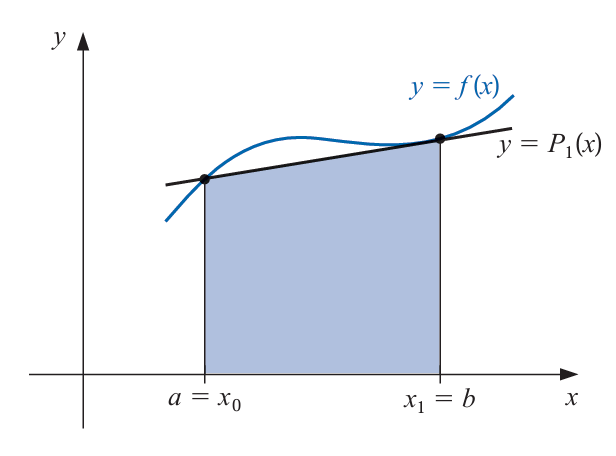
\includegraphics[width=\linewidth]{figures/T} 
    \caption{Trapezoidal rule\cite{PFGPlots}}
    \end{subfigure}
    \begin{subfigure}{0.45\linewidth}
        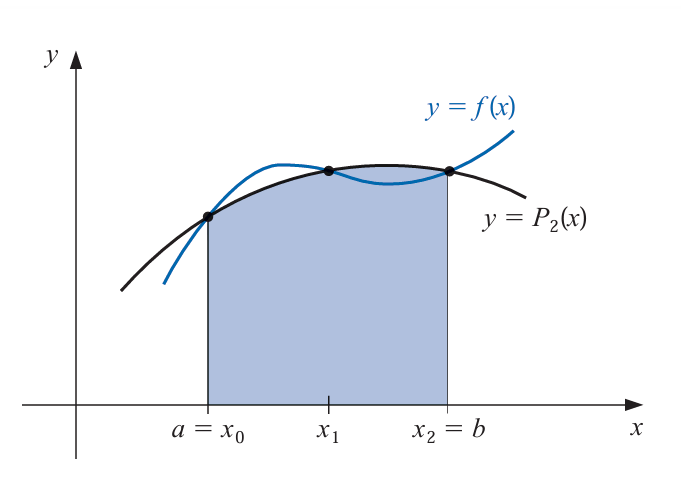
\includegraphics[width=\linewidth]{figures/S} 
        \caption{Simpson's rule}
    \end{subfigure}
\end{figure*}
\begin{figure*}[tp]
    \centering
    \begin{subfigure}{0.45\linewidth}
        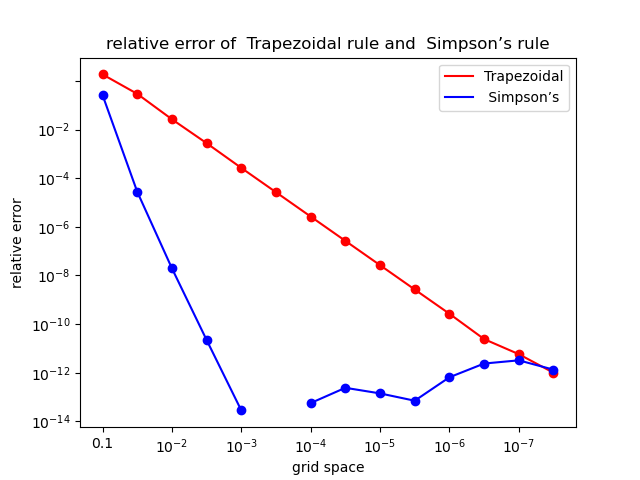
\includegraphics[width=\linewidth]{figures/IntErr.png} 
        \caption{误差}
    \end{subfigure}
    \begin{subfigure}{0.45\linewidth}
    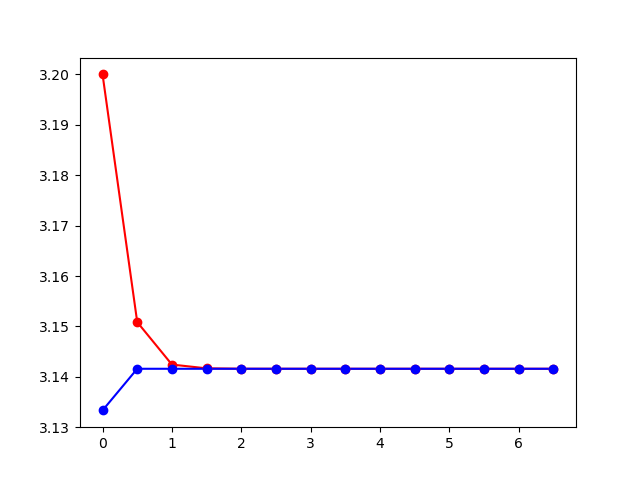
\includegraphics[width=\linewidth]{figures/Int.png} 
    \caption{梯形法和辛普森法在不同格点数下计算的积分值}
    \end{subfigure}

\end{figure*}
\section{Monte Carlo Method}
蒙特卡罗方法又称随机模拟法或统计试验法, 是通过随机变量的统计实验求解数学物理问题的数值
方法. 用蒙特卡罗方法解决实际问题时, 无论是随机性问题或是确定性问题需要把具体问题看做某
一随机事件, 在计算机上选用恰当的数学模型进行模拟. 其基本特点有:
\begin{enumerate}
    \item 程序结构简单, 占内存少
    \item 收敛慢, 但其收敛速度与误差和维数无关, 这是其他方法不具备的优点
    \item 边界条件复杂不带来求解的复杂性
\end{enumerate}
设区间[a,b]中的随机变量𝜉的分布由密度函数f(x)给出,g(x)是定义在[a,b]上的连续函数. 则给$g(\xi)$的数学期望:
\begin{align}
    E(g(\xi))=\int_a^b g(x)f(x)dx
\end{align}
同时,根据大数定律
\begin{align}
    E=\lim_{N\rightarrow \infty}\sum_{i=1}^{N}\frac{g(x_i)}{N}
\end{align}
通常,为了方便计算选择f(x)为均匀分布的概率密度,从而
\begin{align}
    \int_{a}^{b} g(x)dx=(b-a)\int_a^b \frac{g(x)}{b-a}dx=(b-a)\lim_{N\rightarrow \infty}\sum_{i=1}^{N}\frac{g(x_i)}{N}
\end{align}
这个结果不难推广到二维:
\begin{align}
    \iint H(x,y)dxdy=A\iint \frac{H(x,y)}{A}dS=A\lim_{N\rightarrow \infty}\sum_{i=1}^{N}\frac{H(x_i,y_i)}{N}
\end{align}
\newpage
\begin{figure*}[tp]
    \centering
    \begin{subfigure}{0.45\linewidth}
        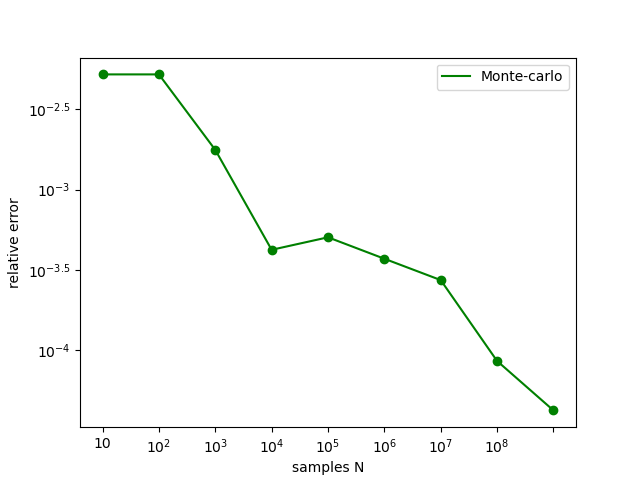
\includegraphics[width=\linewidth]{figures/MCerr.png} 
        \caption{蒙特卡洛法的误差}
    \end{subfigure}
    \begin{subfigure}{0.45\linewidth}
    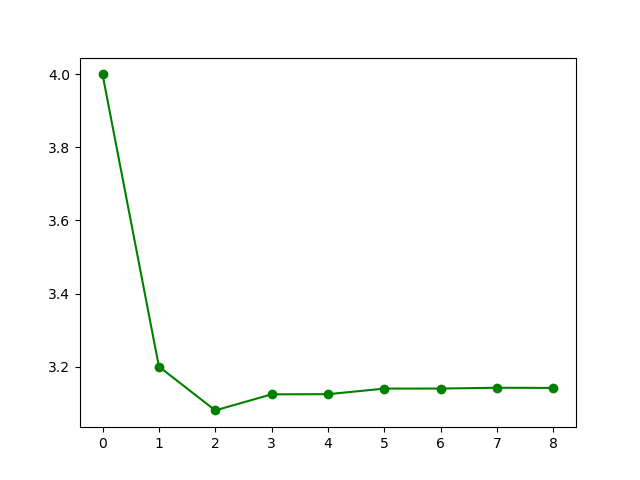
\includegraphics[width=\linewidth]{figures/MC.png} 
    \caption{不同试验次数蒙特卡洛法的积分值}
    \end{subfigure}
\end{figure*}
\begin{tauenv}[frametitle=Example]
    \begin{align}
        \int_{-1}^{1}\int_{-1}^{1} H(x,y)=4\lim_{N\rightarrow \infty}\sum_{i=1}^{N}\frac{H(x_i,y_i)}{N}\\
        H(x,y)(x)=\left\{
            \begin{array}{rl}
            1 & \text{if \qquad} x^2+y^2\leqslant 1\\
            0 & \text{if \qquad} else
            \end{array} \right .\notag
    \end{align}
\end{tauenv}
\nolinenumbers
\lstinputlisting[caption=code, language=Matlab]{code2.py}
\linenumbers
\section{Codes}
以下是全部的实例代码以及matploylib绘图部分:
	\nolinenumbers
	\lstinputlisting[caption=code, language=Matlab]{main.py}
	\linenumbers